\documentclass[a4paper, 12pt, english]{article}

% \usepackage[portuges]{babel}
\usepackage[utf8]{inputenc}
\usepackage{amsmath,amssymb}
\usepackage{graphicx}
\usepackage{subfig}
\usepackage[colorinlistoftodos]{todonotes}

\usepackage{indentfirst}
\usepackage{verbatim}
\usepackage{textcomp}
\usepackage{gensymb}

\usepackage{relsize}

\usepackage{lipsum}% http://ctan.org/pkg/lipsum
\usepackage{xcolor}% http://ctan.org/pkg/xcolor
\usepackage{xparse}% http://ctan.org/pkg/xparse
\NewDocumentCommand{\myrule}{O{1pt} O{2pt} O{black}}{%
  \par\nobreak % don't break a page here
  \kern\the\prevdepth % don't take into account the depth of the preceding line
  \kern#2 % space before the rule
  {\color{#3}\hrule height #1 width\hsize} % the rule
  \kern#2 % space after the rule
  \nointerlineskip % no additional space after the rule
}
\usepackage[section]{placeins}

\usepackage{booktabs}
\usepackage{colortbl}%
   \newcommand{\myrowcolour}{\rowcolor[gray]{0.925}}
   
\usepackage[obeyspaces]{url}
\usepackage{etoolbox}
\usepackage[colorlinks,citecolor=black,urlcolor=blue,bookmarks=false,hypertexnames=true]{hyperref} 

\usepackage{geometry}
\geometry{
	paper=a4paper, % Change to letterpaper for US letter
	inner=3cm, % Inner margin
	outer=3cm, % Outer margin
	bindingoffset=.5cm, % Binding offset
	top=2cm, % Top margin
	bottom=2cm, % Bottom margin
	%showframe, % Uncomment to show how the type block is set on the page
}

\usepackage{amsmath,amsfonts}


\usepackage{multicol,caption}
\newenvironment{Figure}
  {\par\medskip\noindent\minipage{\linewidth}}
  {\endminipage\par\medskip}
\usepackage{array}

\newcommand{\highlight}[1]{\textcolor{blue}{\texttt{#1}}}

\graphicspath{{images/}}

%*******************************************************************************%
%************************************START**************************************%
%*******************************************************************************%
\begin{document}

%************************************TITLE PAGE**************************************%
\begin{titlepage}
\begin{center}
\textbf{\LARGE Alexandria University}\\[0.5cm] 
\textbf{\large FACULTY OF ENGINEERING}\\[0.2cm]
\vspace{20pt}

\includegraphics{logo.png}\\[1cm]
\par
\vspace{20pt}
\textbf{\Large EEC332 Analog Integrated Circuits}\\
\vspace{15pt}
\myrule[1pt][7pt]
\textbf{\LARGE  Experiment 1}\\
\vspace{15pt}
\textbf{\large Study the characteristics of negative feedback amplifiers and design of an instrumentation amplifier}\\
\myrule[1pt][7pt]
\vspace{25pt}
\textbf{\large \hspace{50pt}Student Name \hspace{60pt} Student ID}\\
Ahmed Osama Mohamed Afifi \hspace{60pt} 20010038 \\
Ziad Mohamed Mohamed Abdalla \hspace{40pt} 20010643 \\

\vspace{45pt}
%\textbf {\large Lecturer in charge:}\\[0.2cm]
%\Large {Ir. Chan Cheong Loong}\\[0.1cm]
\end{center}

\par
\vfill
\begin{center}
\textbf{Submission Date : 16/03/2024}\\
\end{center}

\end{titlepage}

%************************************TABLE OF CONTENTS**************************************%

%  %Sumário
%  \newpage
%  \tableofcontents
%  \thispagestyle{empty}
%  %End Sumário

%********************************%
%***********SECTION 1************%
%********************************%
\newpage
\section{Introduction}
An OP-Amp can be used in negative feedback mode to build unity gain amplifiers, non-inverting amplifiers and inverting amplifiers. While an ideal OP-Amp is assumed to have infinite open-loop gain and infinite bandwidth, real OP-Amps have finite numbers for these parameters. Therefore, it is important to understand some limitations of real OP-Amps, such as finite Gain-Bandwidth Product (GB). Similarly, the slew rate and saturation limits of an operational amplifier are equally important.
\newline

%********************************%
%***********SECTION 2************%
%********************************%
\section{Unity Gain Amplifier}
\subsection{Schematic}
\begin{Figure}
 \centering
 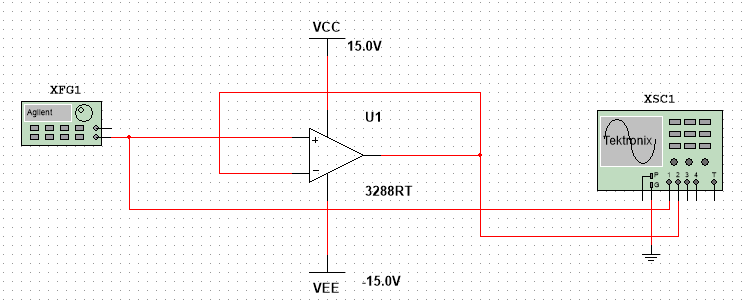
\includegraphics[width=1.2\linewidth, scale=2]{images/unityGainSchematic.png}
 \captionof{figure}{A unity gain system}
\end{Figure}

\subsection{Input parameters}
\begin{multicols}{2}
\begin{tabular}{>{\raggedright}p{\linewidth} >{\raggedleft}p{\linewidth}}
\begin{Figure}
 \centering
 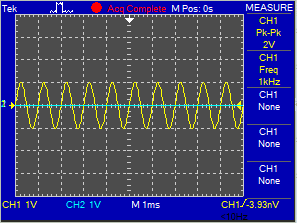
\includegraphics[width=\linewidth, scale=2]{images/inputSignalSine.png}
 \captionof{figure}{Input signal (sinusoidal)}
\end{Figure} & 
\begin{Figure}
 \centering
 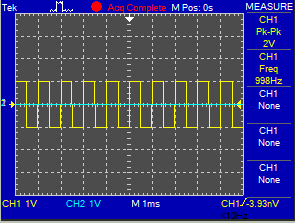
\includegraphics[width=\linewidth, scale=2]{images/inputSignalSquare.png}
 \captionof{figure}{Input signal (square)}
\end{Figure}
\end{tabular}
\end{multicols}
\newpage

\subsection{Results}
\subsubsection{Lab results}
\begin{figure}[h]
    \centering
    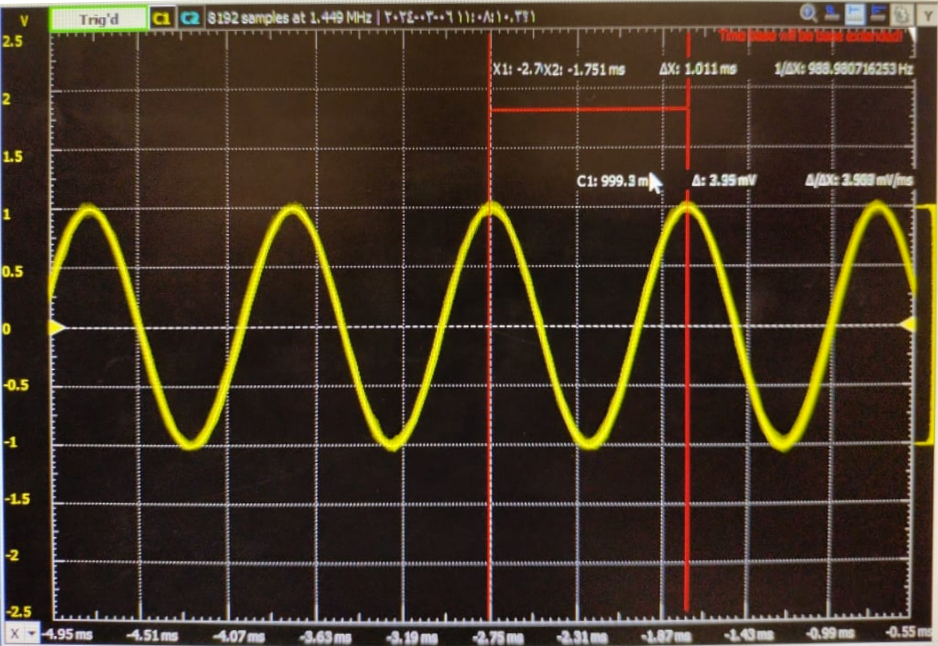
\includegraphics[width=\linewidth]{images/unityLab.png}
    \caption{Lab result for unity gain amplifier}
    \label{fig:Lab result for unity gain amplifier}
\end{figure}
\subsubsection{Simulation results}
\begin{multicols}{2}
\begin{tabular}{>{\raggedright}p{\linewidth} >{\raggedleft}p{\linewidth}}
\begin{Figure}
 \centering
 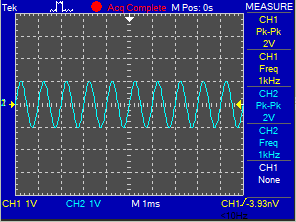
\includegraphics[width=\linewidth, scale=2]{images/unitySinSim.png}
 \captionof{figure}{Sinusoidal output}
\end{Figure} & 
\begin{Figure}
 \centering
 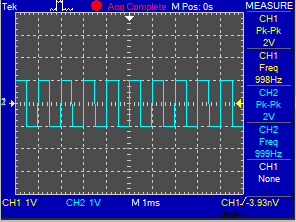
\includegraphics[width=\linewidth, scale=2]{images/unitySquareSim.png}
 \captionof{figure}{Square Output}
\end{Figure}
\end{tabular}
\end{multicols}

\begin{Figure}
 \centering
 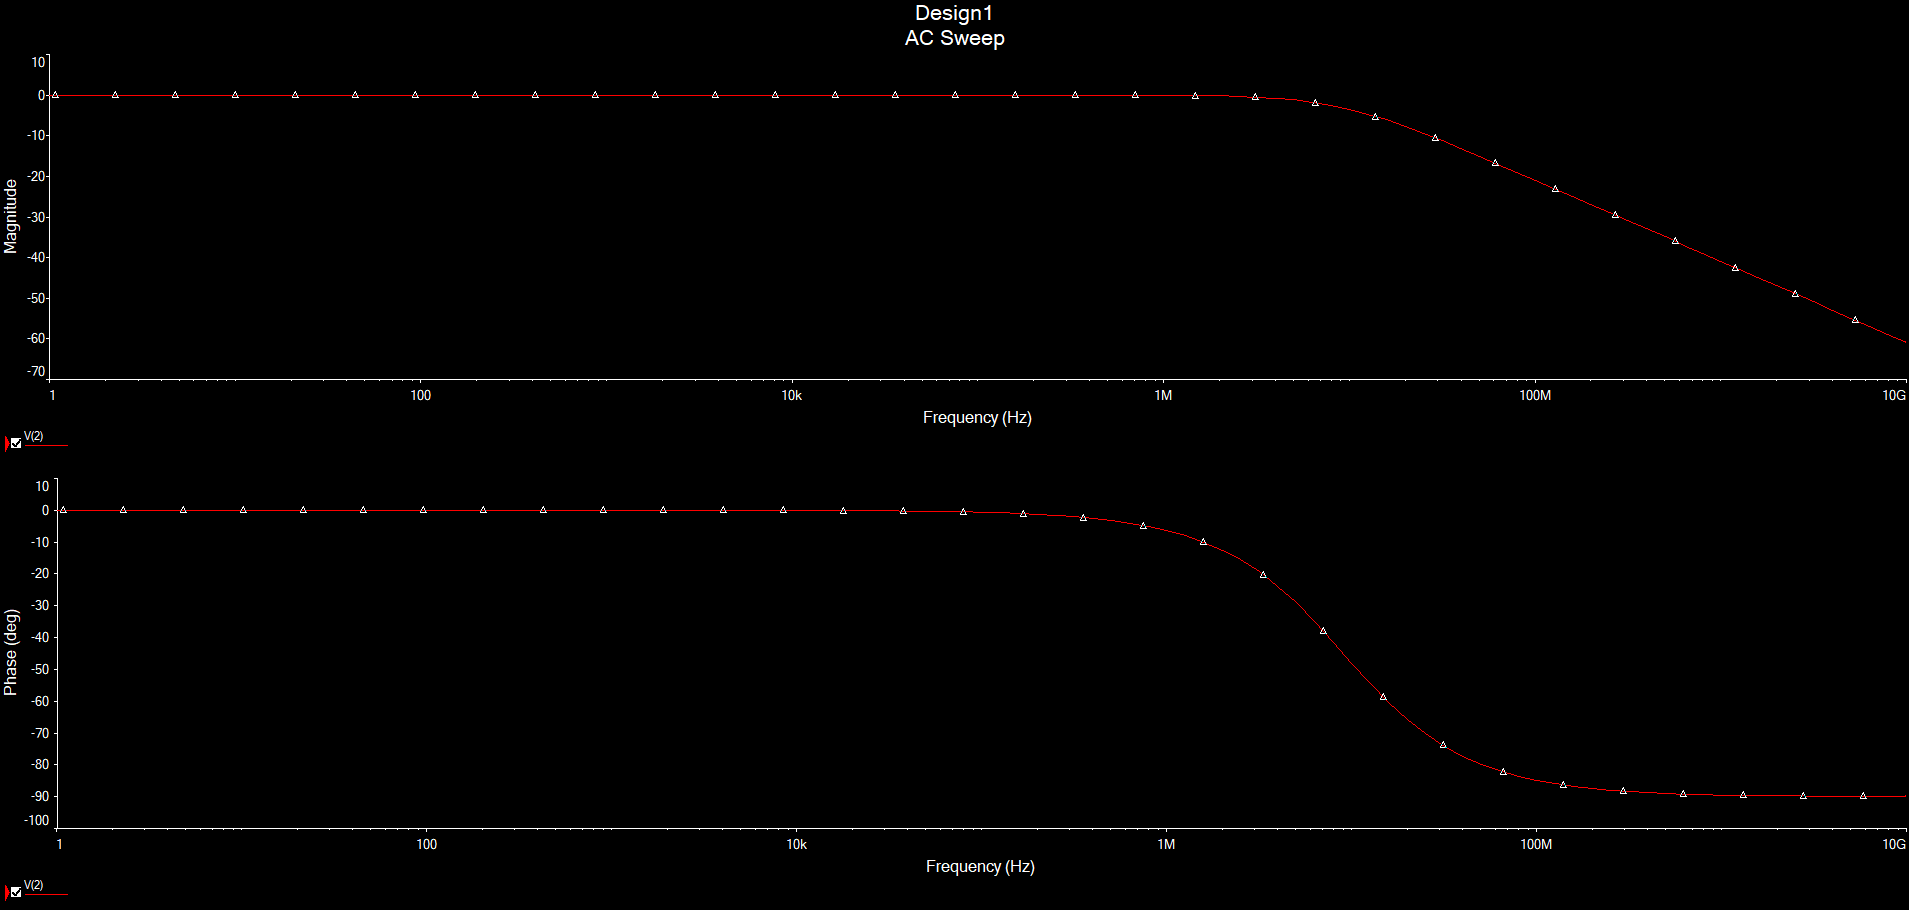
\includegraphics[width=\linewidth, scale=2]{images/unityFrequencyResponseSin.png}
 \captionof{figure}{Frequency Response}
\end{Figure}

\subsection{Comments}
In unity gain amplifiers, the output signal is the same as the input signal. Since \( V_{out} = A_{\nu}V_{in} \), and the gain is unity. Therefore, \( V_{out} = V_{in} \).

\newpage
%********************************%
%***********SECTION 3************%
%********************************%
\section{Non-Inverting Amplifier}
\subsection{Schematic}
\begin{Figure}
 \centering
 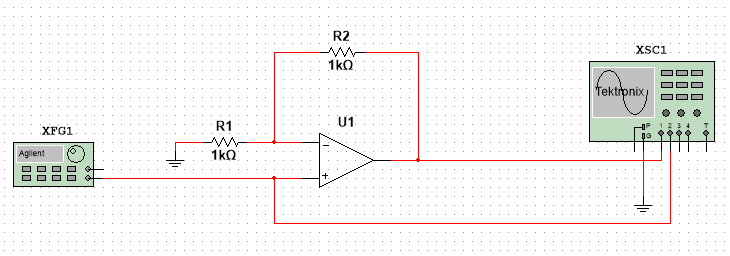
\includegraphics[width=1.2\linewidth, scale=2]{images/nonInvertingSchematic.png}
 \captionof{figure}{Non-Inverting gain system}
\end{Figure}

\subsection{Input parameters}
\begin{multicols}{2}
\begin{tabular}{>{\raggedright}p{\linewidth} >{\raggedleft}p{\linewidth}}
\begin{Figure}
 \centering
 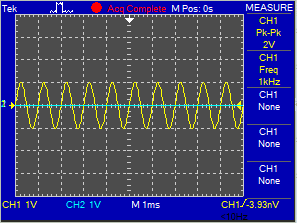
\includegraphics[width=\linewidth, scale=2]{images/inputSignalSine.png}
 \captionof{figure}{Input signal (sinusoidal)}
\end{Figure} & 
\begin{Figure}
 \centering
 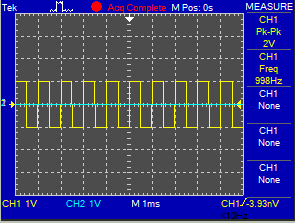
\includegraphics[width=\linewidth, scale=2]{images/inputSignalSquare.png}
 \captionof{figure}{Input signal (square)}
\end{Figure}
\end{tabular}
\end{multicols}
\newpage

\subsection{Results}
\subsubsection{Lab results}
\begin{figure}[h]
    \centering
    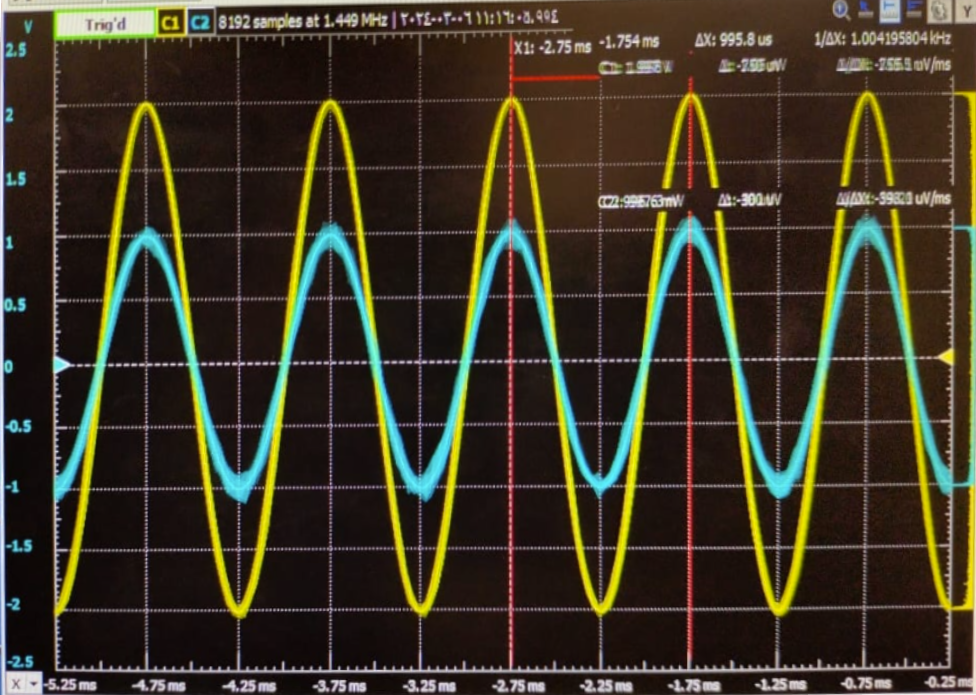
\includegraphics[width=\linewidth]{images/nonInvertLab.png}
    \caption{Lab result for non inverting amplifier}
    \label{fig:Lab result for non inverting amplifier}
\end{figure}
\subsubsection{Simulation results}
\begin{multicols}{2}
\begin{tabular}{>{\raggedright}p{\linewidth} >{\raggedleft}p{\linewidth}}
\begin{Figure}
 \centering
 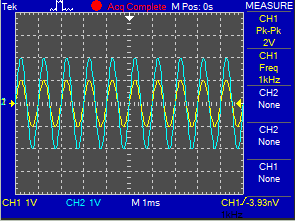
\includegraphics[width=\linewidth, scale=2]{images/nonInvertSinSim.png}
 \captionof{figure}{Sinusoidal output}
\end{Figure} & 
\begin{Figure}
 \centering
 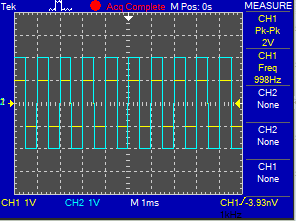
\includegraphics[width=\linewidth, scale=2]{images/nonInvertSquareSim.png}
 \captionof{figure}{Square Output}
\end{Figure}
\end{tabular}
\end{multicols}

\begin{Figure}
 \centering
 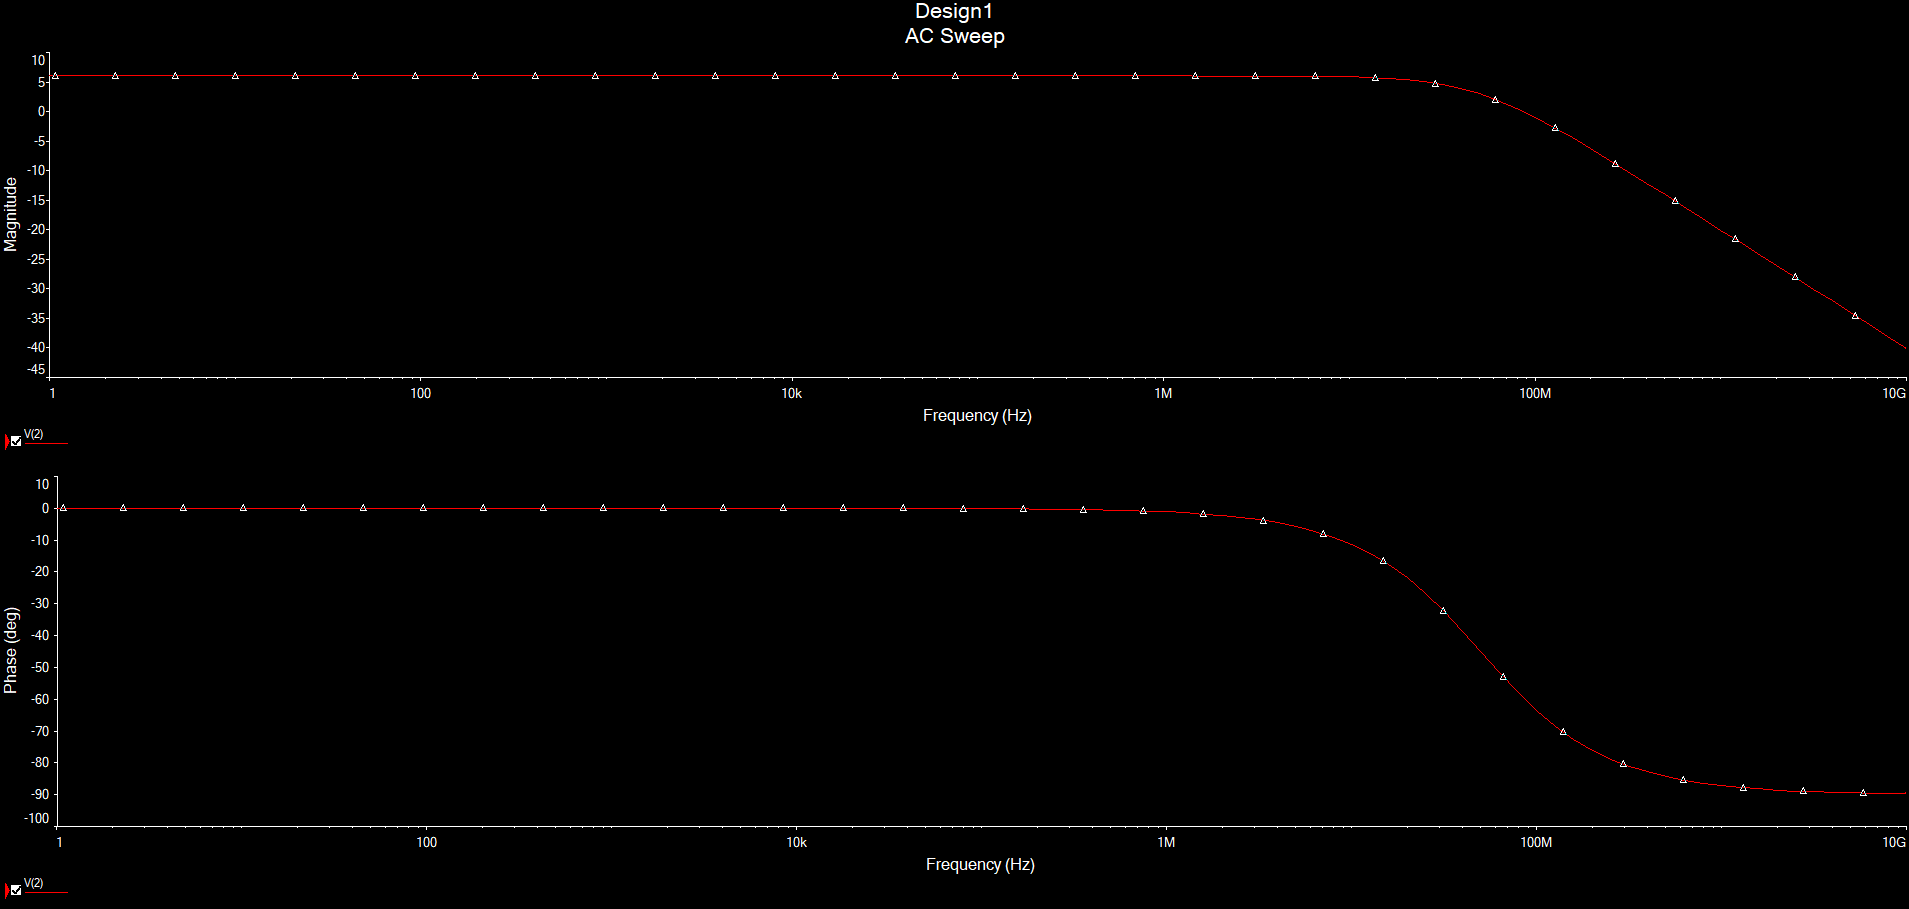
\includegraphics[width=\linewidth, scale=2]{images/nonInvertFrequencyResponseSin.png}
 \captionof{figure}{Frequency Response}
\end{Figure}

\subsection{Comments}
In non-inverting amplifiers, the gain is given as \( A_{\nu} = 1 + \frac{R_{2}}{R_{1}} \). Thus, the gain depends on the ratio between the feedback resistance and the input resistance. Since the two resistors are equal. Therefore, the gain \( A_{\nu} = 2 \), and the output voltage \( V_{out} = 2V_{in} \).

\newpage
%********************************%
%***********SECTION 4************%
%********************************%
\section{Inverting Amplifier}
\subsection{Schematic}
\begin{Figure}
 \centering
 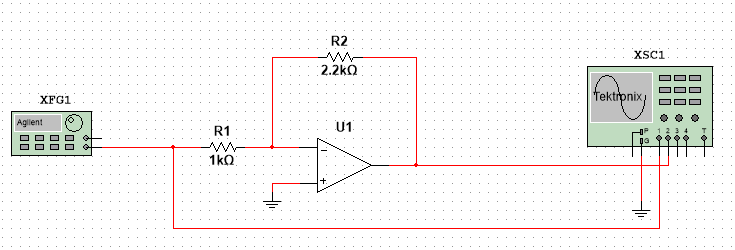
\includegraphics[width=1.2\linewidth, scale=2]{images/invertingSchematic.png}
 \captionof{figure}{Inverting gain system}
\end{Figure}


\subsection{Input parameters}
\begin{multicols}{2}
\begin{tabular}{>{\raggedright}p{\linewidth} >{\raggedleft}p{\linewidth}}
\begin{Figure}
 \centering
 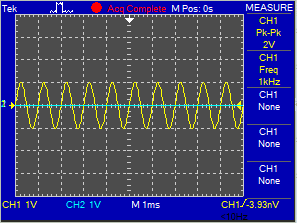
\includegraphics[width=\linewidth, scale=2]{images/inputSignalSine.png}
 \captionof{figure}{Input signal (sinusoidal)}
\end{Figure} & 
\begin{Figure}
 \centering
 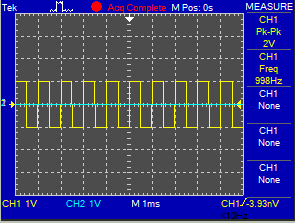
\includegraphics[width=\linewidth, scale=2]{images/inputSignalSquare.png}
 \captionof{figure}{Input signal (square)}
\end{Figure}
\end{tabular}
\end{multicols}
\newpage

\subsection{Results}
\subsubsection{Lab results}
\begin{figure}[h]
    \centering
    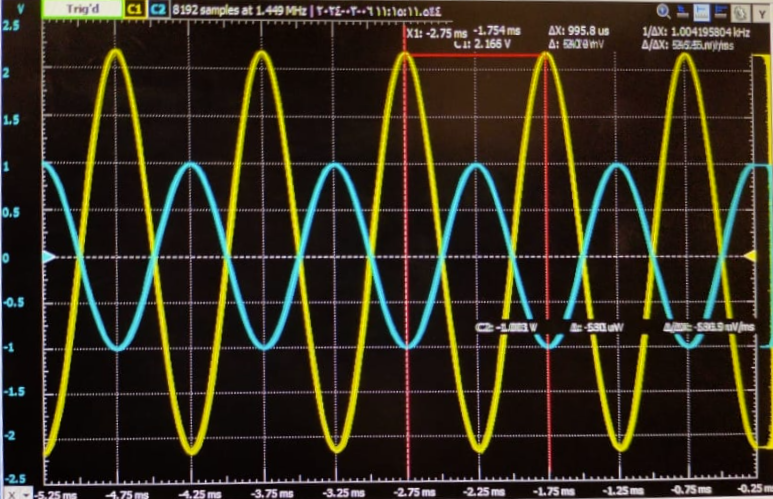
\includegraphics[width=\linewidth]{images/invertingLab.png}
    \caption{Lab result for inverting amplifier}
    \label{fig:Lab result for inverting amplifier}
\end{figure}
\subsubsection{Simulation results}
\begin{multicols}{2}
\begin{tabular}{>{\raggedright}p{\linewidth} >{\raggedleft}p{\linewidth}}
\begin{Figure}
 \centering
 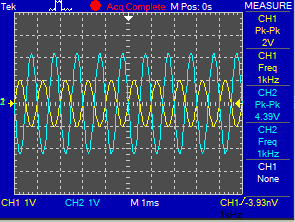
\includegraphics[width=\linewidth, scale=2]{images/invertingSinSim.png}
 \captionof{figure}{Sinusoidal output}
\end{Figure} & 
\begin{Figure}
 \centering
 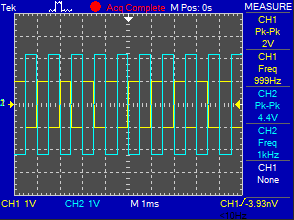
\includegraphics[width=\linewidth, scale=2]{images/invertingSquareSim.png}
 \captionof{figure}{Square Output}
\end{Figure}
\end{tabular}
\end{multicols}

\begin{Figure}
 \centering
 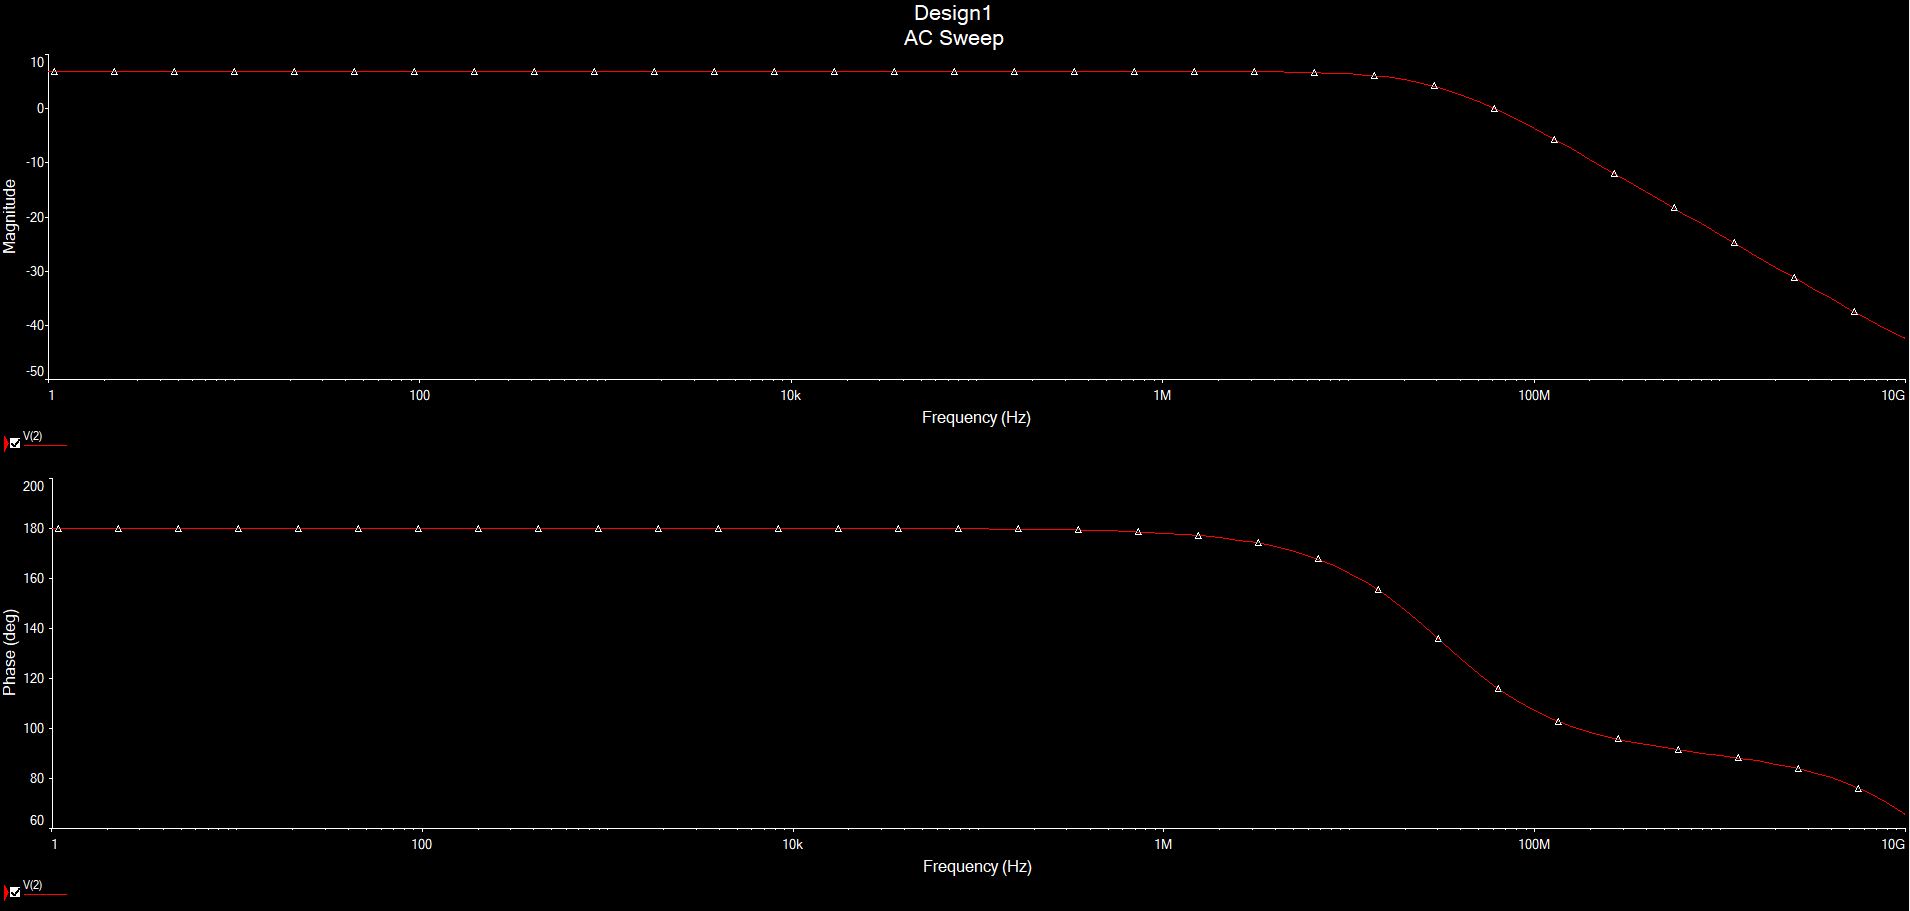
\includegraphics[width=\linewidth, scale=2]{images/invertingFrequencyResponseSin.png}
 \captionof{figure}{Frequency Response}
\end{Figure}

\subsection{Comments}
In inverting amplifiers, the gain is given as \( A_{\nu} = -\frac{R_{2}}{R_{1}} \). Thus, the gain depends on the ratio between the feedback resistance and the input resistance, and the negative sign represents a phase shift between the output signal and the input signal. As the feedback resistance \( R_{2} = 2.2k\ohm \), and the input resistance \( R_{1} = 1k\ohm \), the gain \( |A_{\nu}| = 2.2 \) and the output voltage \( |V_{out}| = 2.2|V_{in}| \) and there is a phase shift of $\pi$ between the two signals.

\newpage
%********************************%
%***********SECTION 5************%
%********************************%
\section{Instrumentation Amplifier}
\subsection{Instrumentation Amplifier with three amplifiers}
\subsubsection{Schematic}
\begin{Figure}
 \centering
 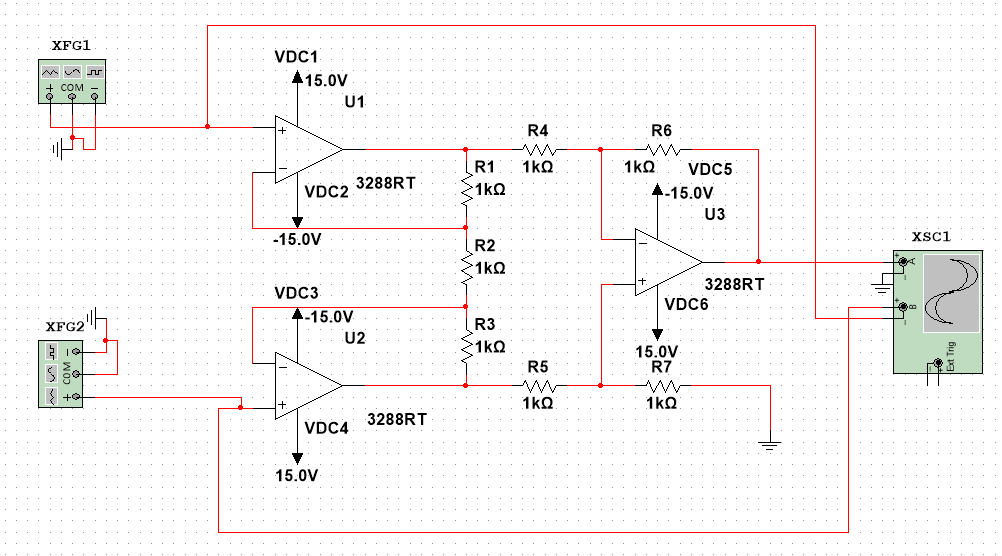
\includegraphics[width=1.2\linewidth, scale=2]{images/Instrumentation3opamp circuit.png}
 \captionof{figure}{Instrumentation Amplifier with three amplifiers}
\end{Figure}

\subsubsection{Results}
\begin{multicols}{2}
\begin{tabular}{>{\raggedright}p{\linewidth} >{\raggedleft}p{\linewidth}}
\begin{Figure}
 \centering
 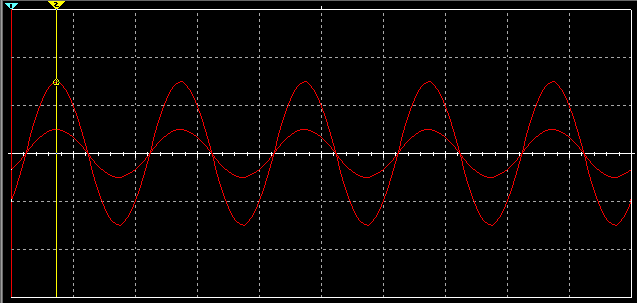
\includegraphics[width=\linewidth, scale=2]{images/3ampsSin.png}
 \captionof{figure}{Sin wave}
\end{Figure} & 
\begin{Figure}
 \centering
 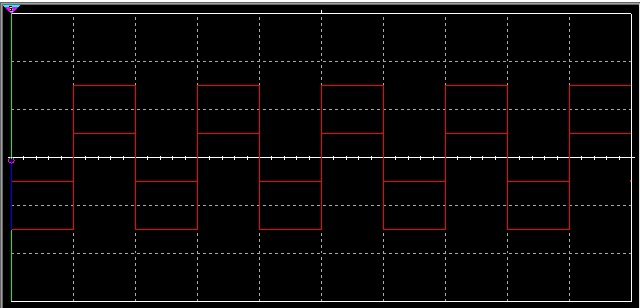
\includegraphics[width=\linewidth, scale=2]{images/3ampsSquare.png}
 \captionof{figure}{Input signal (square)}
\end{Figure}
\end{tabular}
\end{multicols}
\subsubsection{Frequency Response}
\begin{Figure}
 \centering
 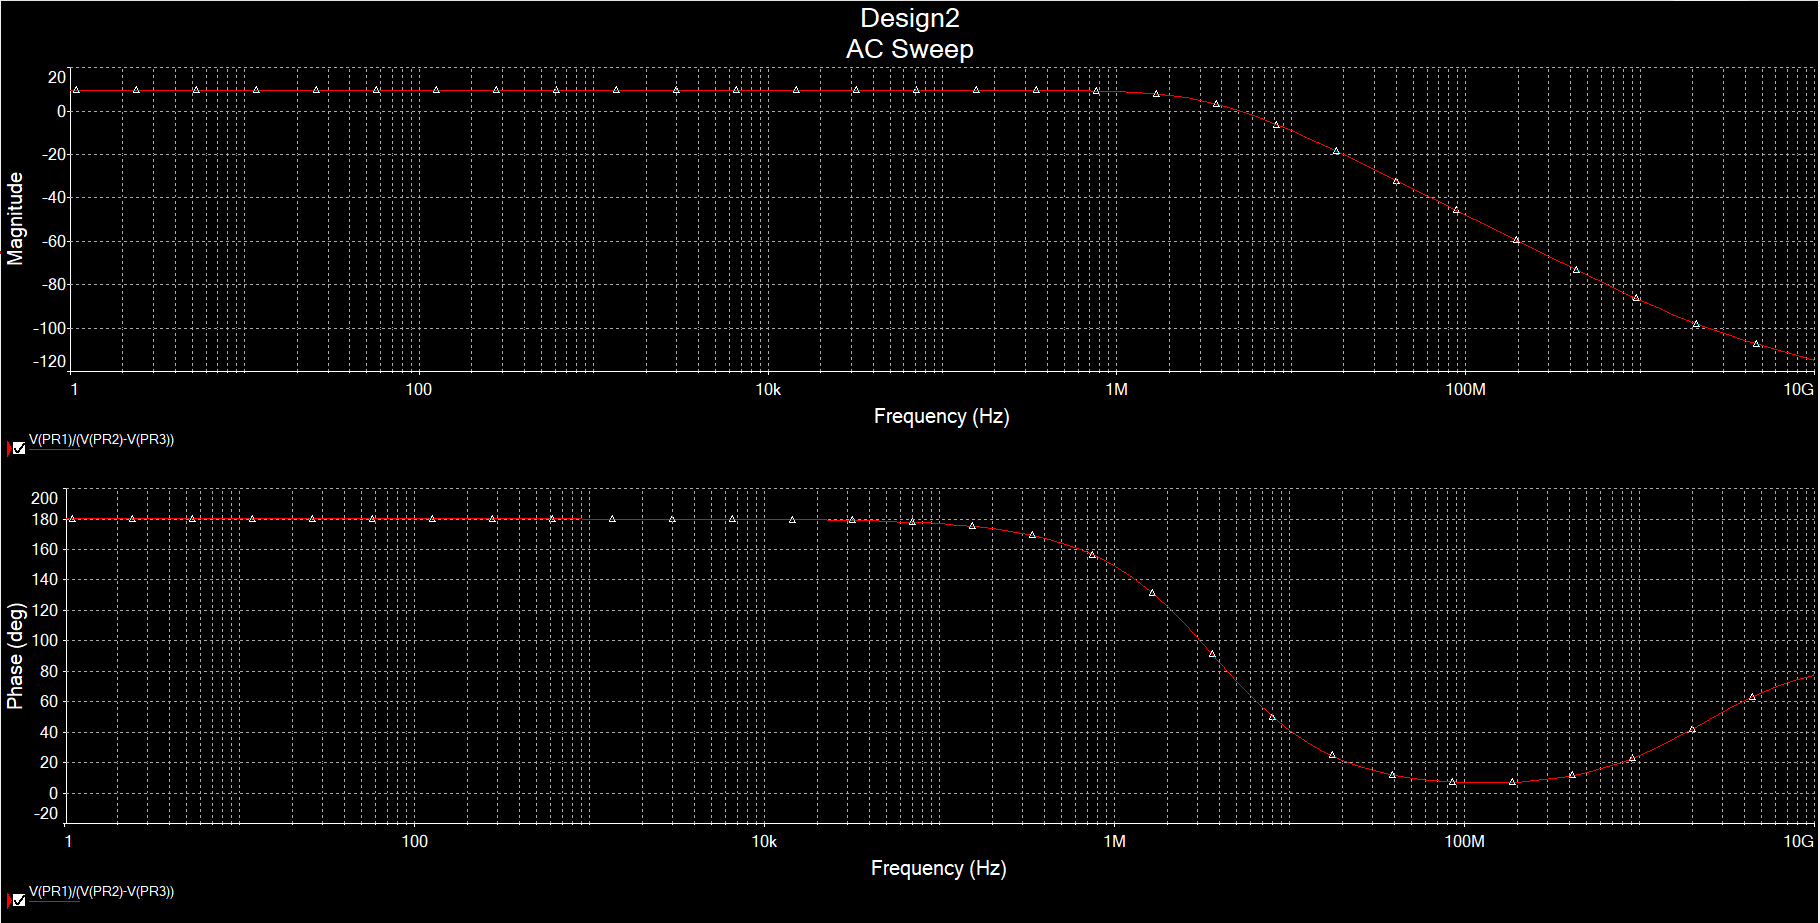
\includegraphics[width=1.2\linewidth, scale=2]{images/instu freq res.png}
 \captionof{figure}{Frequency Response}
\end{Figure}

\subsubsection{Comments}
The gain in this case is \(A_{\nu}=(1+\frac{2R_{2}}{R_{gain}})\frac{R_{4}}{R_{3}} = 3\). Therefore, to get $R_{g}$ with the assumption that $R_{1} = R_{2} = 1k\ohm$.


\subsection{Instrumentation Amplifier with two amplifiers}
\subsubsection{Schematic}
\begin{Figure}
 \centering
 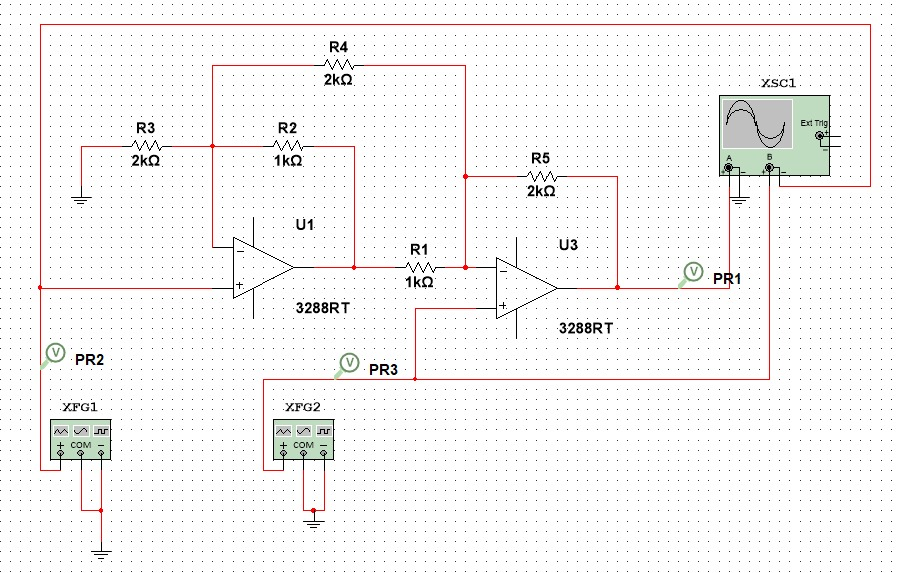
\includegraphics[width=1.2\linewidth, scale=2]{images/Instrumentation2amps.png}
 \captionof{figure}{Instrumentation Amplifier with two amplifiers}
\end{Figure}
\subsubsection{Results}
\begin{multicols}{2}
\begin{tabular}{>{\raggedright}p{\linewidth} >{\raggedleft}p{\linewidth}}
\begin{Figure}
 \centering
 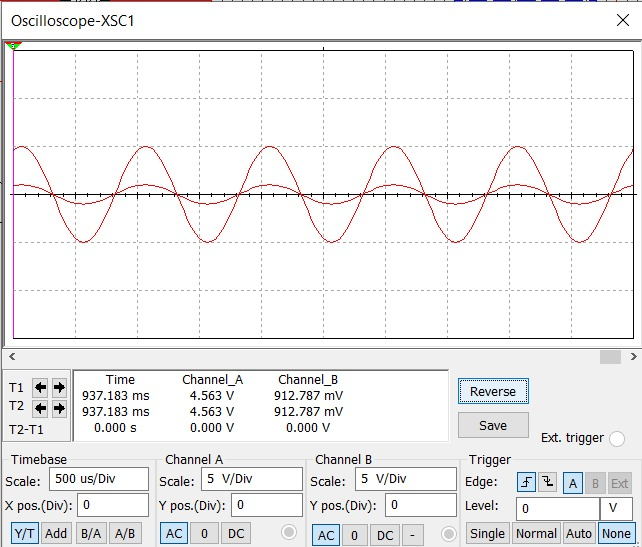
\includegraphics[width=\linewidth, scale=2]{images/2ampsSin.png}
 \captionof{figure}{Sin wave}
\end{Figure} & 
\begin{Figure}
 \centering
 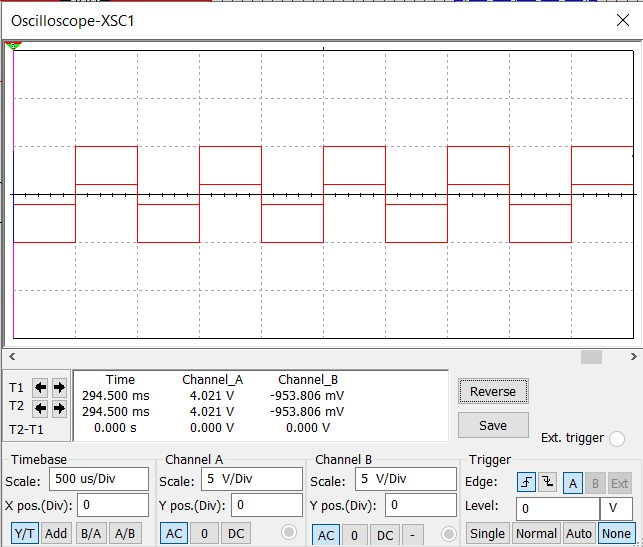
\includegraphics[width=\linewidth, scale=2]{images/2ampsSquare.png}
 \captionof{figure}{Square wave}
\end{Figure}
\end{tabular}
\end{multicols}

\subsubsection{Frequency Response}
\begin{Figure}
 \centering
 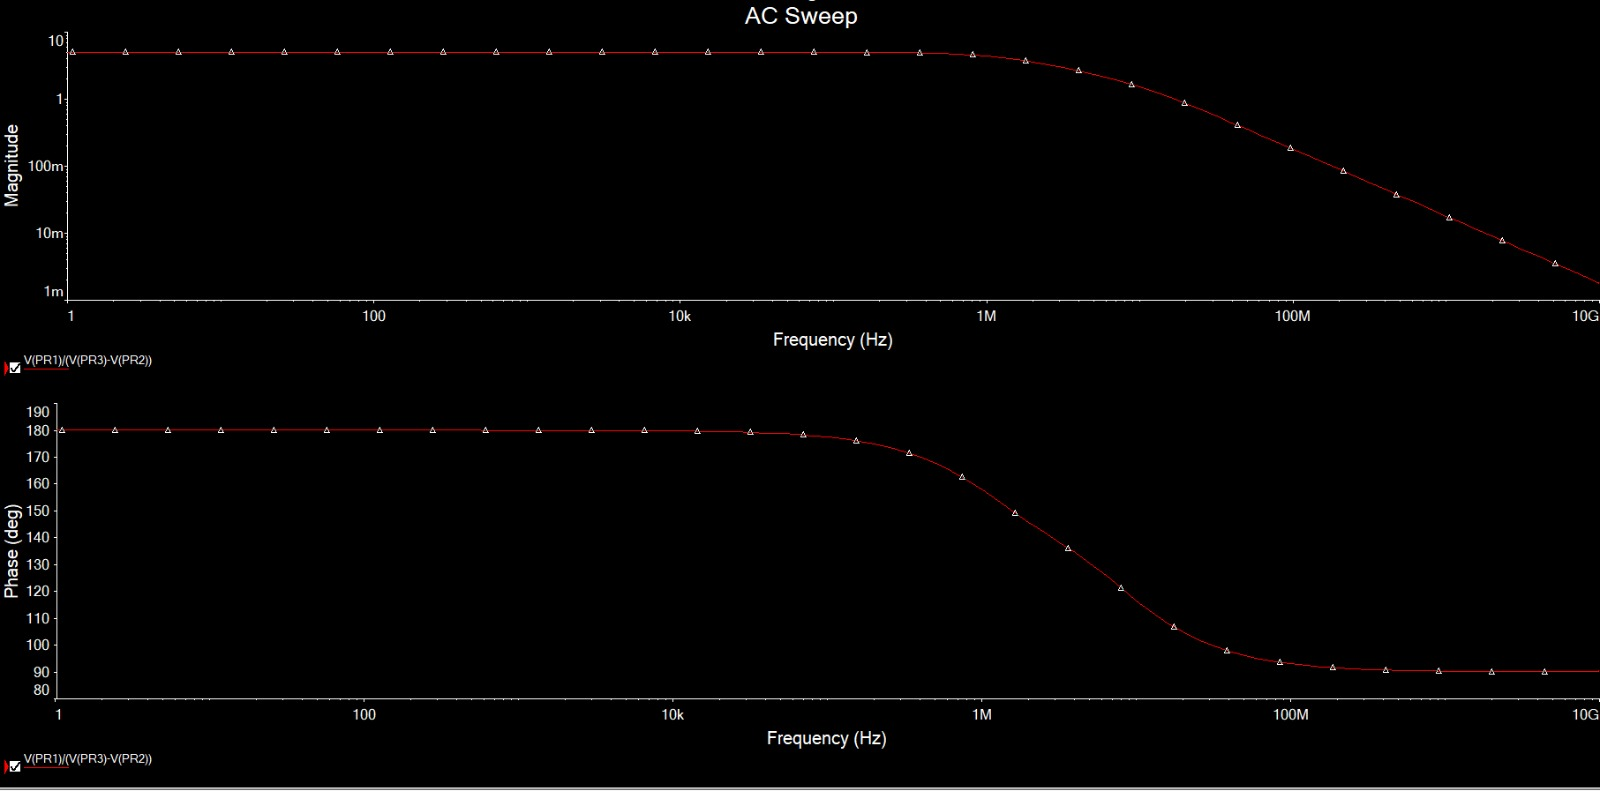
\includegraphics[width=1.2\linewidth, scale=2]{images/2ampsFR.png}
 \captionof{figure}{Frequency Response}
\end{Figure}

\subsubsection{Comments}
The gain in this case is \(A_{\nu}=1+\frac{R_{2}}{R_{1}}+\frac{2R_{2}}{R_{gain}} = 5\). Therefore, to get $R_{g}$ with assumption that $R_{1} = 1k\ohm$ and $R_{2} = 2k\ohm$ we will get $R_{g} = 2k\ohm$.


\patchcmd{\thebibliography}{\section*}{\section}{}{}

\end{document}